\documentclass[12]{article}

%import packages for theoretical computer science stuff
\usepackage{amsmath}
\usepackage{amssymb}
\usepackage{amsthm}
\usepackage{mathrsfs}

%import packages for images
\usepackage{graphicx}
\usepackage{float}

%import packages for algorithms
\usepackage{algorithm}
\usepackage{algorithmic}
\usepackage{listings}



%setup document margins and spacing
\usepackage[margin=1in]{geometry}
\usepackage{setspace}
\onehalfspacing


%import packages for hyperlinks
\usepackage{hyperref}
\hypersetup{
    colorlinks=true,
    linkcolor=purple,
    filecolor=magenta,
    urlcolor=cyan,
}

%begin document
\begin{document}

\begin{titlepage}
    \begin{center}
        \textsc{\LARGE University of Calabria}\\[1.5cm]
        \textsc{\Large Department of Mathematics and Computer Science}\\[0.5cm]
        \textsc{\large Master's Degree in Computer Science}\\[0.5cm]
        \textsc{\large Machine Learning}\\[0.5cm]
    \end{center}
\end{titlepage}

\title{Machine Learning - House Prices Analysis}
%insert 5 members of the group
\author{Daniele Avolio\\
    \and
    Alessandro Fazio\\
    \and
    Merem Hassem Indiris\\
    \and
    Michele Vitale\\
    \and
    Lorenzo Piro\\}
\date{A.Y. 2022/2023}

\maketitle

\begin{figure}[h!]
    \centering
    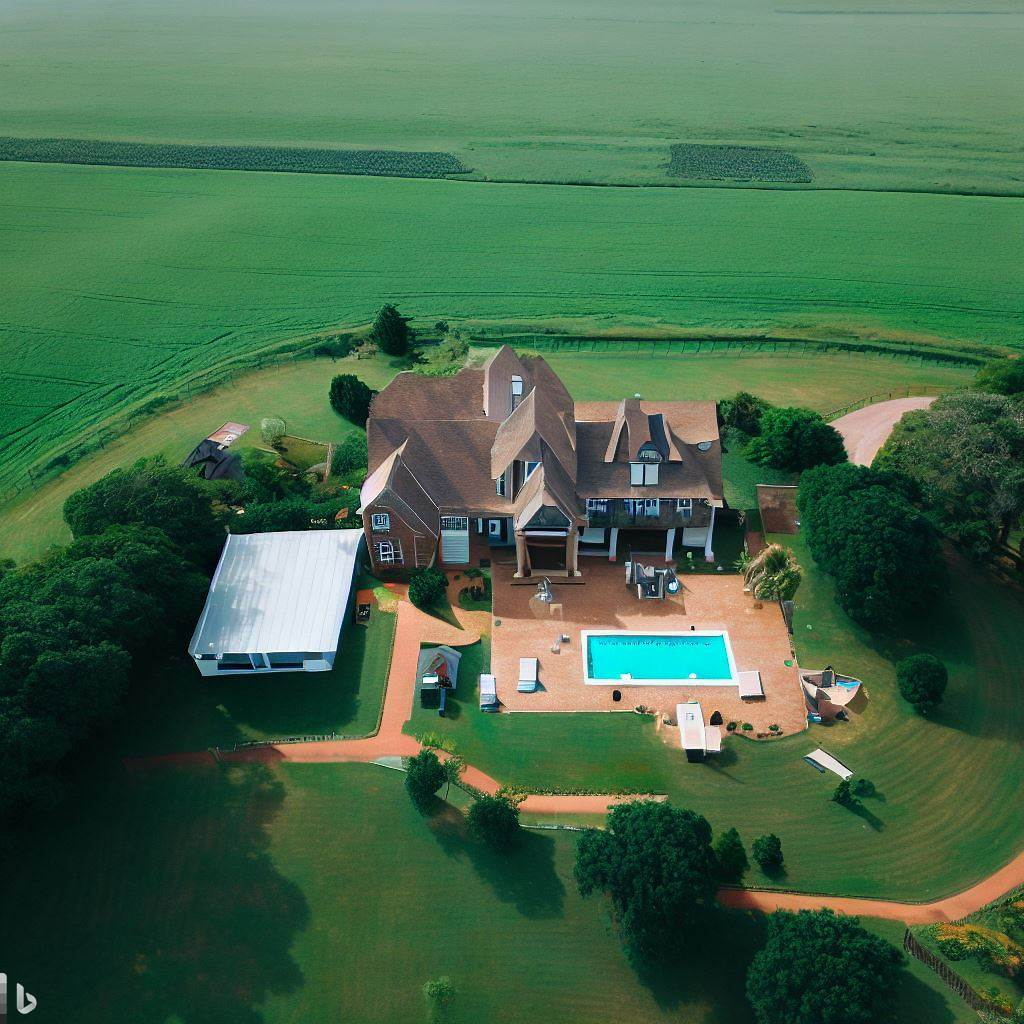
\includegraphics[width=0.6\textwidth]{imgs/house.jpeg}
\end{figure}
\newpage



\chapter{Introduction}
\label{sec:introduction}

To develop this \textbf{Machine Learning} project we are going to use the CRISP-DM methodology, which is a well-known and widely used methodology for data mining projects. It is an iterative process that is composed of six phases.

In particulal, the phases are:
\begin{enumerate}
    \item \textbf{Business Understanding}: in this phase we will try to understand the problem and the objectives of the project. We will also try to understand the data that we have at our disposal and how we can use it to solve the problem.
    \item \textbf{Data Understanding}: in this phase we will try to understand the data that we have at our disposal. We will try to understand the meaning of the data and how we can use it to solve the problem.
    \item \textbf{Data Preparation}: in this phase we will try to prepare the data for the next phases. We will try to clean the data and to transform it in a way that will be useful for the next phases.
    \item \textbf{Modeling}: in this phase we will try to build a model that will be able to solve the problem. We will try to find the best model for our problem.
    \item \textbf{Evaluation}: in this phase we will try to evaluate the model that we have built. We will try to understand if the model is good enough to solve the problem.
    \item \textbf{Deployment}: in this phase we will try to deploy the model that we have built. We will try to understand how we can use the model to solve the problem.
\end{enumerate}

\begin{figure}[H]
    \centering
    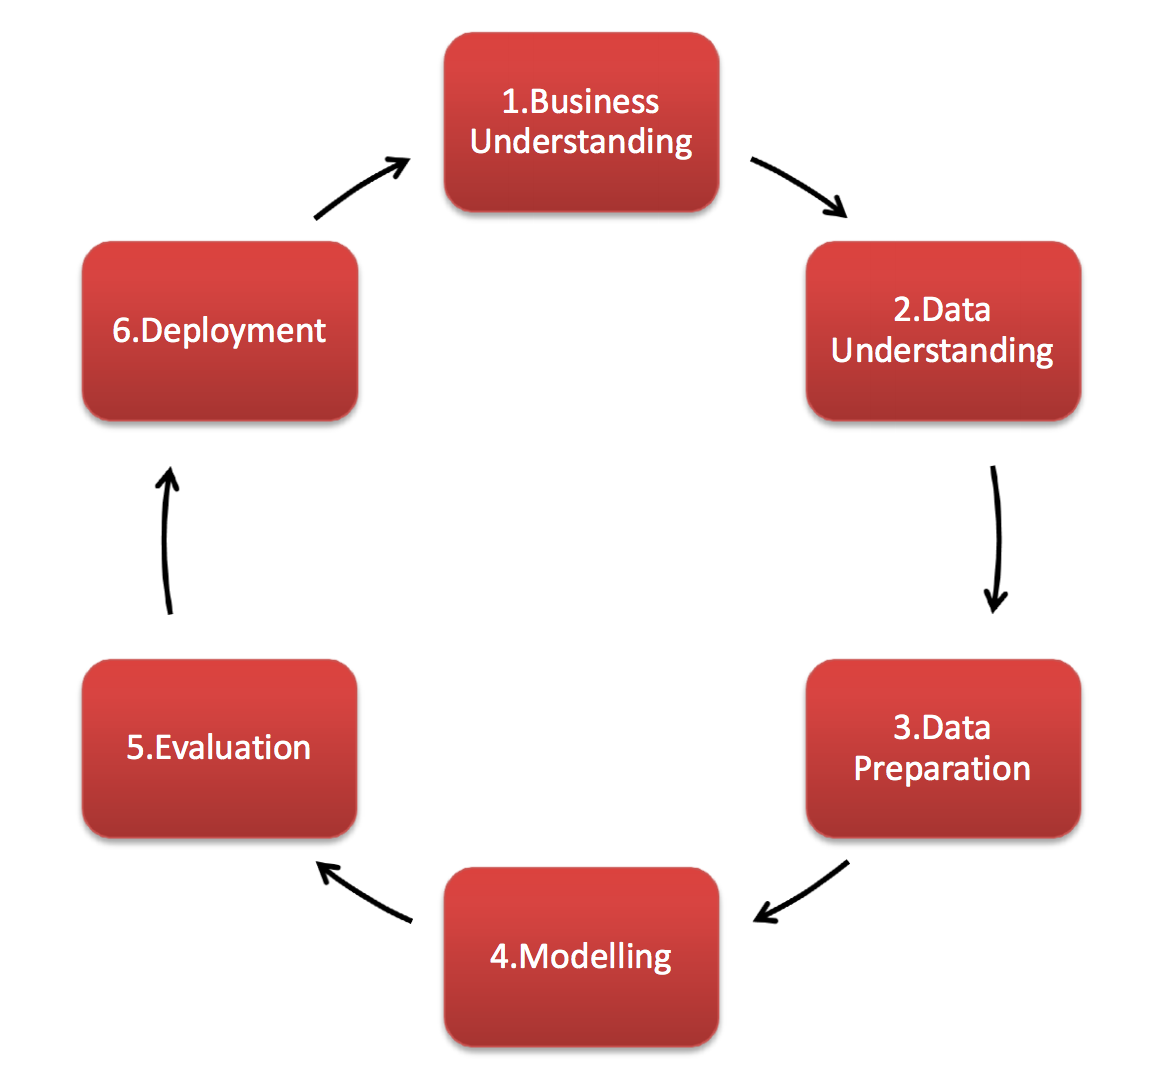
\includegraphics[width=0.5\textwidth]{imgs/crisp.png}
    \caption{CRISP-DM methodology}
    \label{fig:crisp-dm}
\end{figure}
\newpage

\chapter{Business understanding}
\label{sec:business_understanding}

\section{Background}
Our project is based using the dataset of the Kaggle competition \href{https://www.kaggle.com/c/house-prices-advanced-regression-techniques}{House Prices: Advanced Regression Techniques}. 

The goal of the competition is to predict the final price of each home based on 79 explanatory variables describing (almost) every aspect of residential homes in Ames, Iowa.
The dataset is composed by 1460 rows and 81 columns, with an ID column and the last one which is the target variable, the Sale Price.

A small list of the variables is the following:

\begin{itemize}
    \item \textbf{LotArea}: Lot size in square feet
    \item \textbf{OverallQual}: Overall material and finish quality
    \item \textbf{OverallCond}: Overall condition rating
    \item \textbf{YearBuilt}: Original construction date
    \item \textbf{YearRemodAdd}: Remodel date
    \item \textbf{RoofStyle}: Type of roof
    \item \textbf{Exterior1st}: Exterior covering on house
    \item \textbf{Exterior2nd}: Exterior covering on house (if more than one material)
    \item \textbf{MasVnrType}: Masonry veneer type
    \item \textbf{MasVnrArea}: Masonry veneer area in square feet
    \item \dots
\end{itemize}
\section{Business objectives}
\label{subsec:business_objectives}

In this part we are going to analyze the business objective of the project.
Our goal is different from the one of the competition, in fact we are requested to \textbf{convert the Sale Price variable into 3 ranges}:

\begin{enumerate}
    \item \textbf{LOW}: From 0 to 150000 
    \item \textbf{MEDIUM}: From 150000 to 300000 
    \item \textbf{HIGH}: From 300000 and beyond 
\end{enumerate}

So, our goal is to predict a categorical variable with 3 possible values, instead of a continuous variable. 
This is a very important difference, because we are not interested in the exact value of the Sale Price, but only in the range in which it falls.

\section{Business success criteria}
\label{subsec:business_success_criteria}
The success criteria of the project is to obtain a model that is able to predict the Sale Price range with a good accuracy. In particular, we want to create a model that is able to predict the Sale Price range with an accuracy of at least 0.8.

\section{Assessment of the situation}
\label{subsec:assessment_of_the_situation}

There is a very important aspect that we have to consider: there are a lot of variables in the dataset that contains a values of \textbf{NA}, that could leat to thinking that the value is missing.

Actually, this is not always true. In particular, the description of the dataset contains information about the meaning of the \textbf{NA} value for each variable. For example, the \textbf{NA} value for the \textbf{PoolQC} variable means that the house doesn't have a pool, so the value is not missing, but it is a value that has a meaning.

There are more variables that have a similar meaning for the \textbf{NA} value, so we have to be careful when we are going to handle the missing values. For this project, we are going to assume that the \textbf{NA} value is not missing but is just a value that has a meaning. If we need to drop the column, will be specified in the particular section

\section{Inventory of resources}
\label{subsec:inventory_of_resources}

For this project, we are going to use the following resources:

\begin{itemize}
    \item \textbf{Python 3.10.6}: The programming language used for the project
    \item \textbf{Jupyter Notebook}: The IDE used for the project
    \item \textbf{Pandas}: used for data manipulation
    \item \textbf{Numpy}: used for data manipulation
    \item \textbf{Matplotlib}: used for data visualization
    \item \textbf{Seaborn}: used for data visualization
    \item \textbf{Scikit-learn}: used for machine learning 
\end{itemize}

\section{Project Plan}
\label{subsec:project_plan}

The development of the project will be divided into 5 main phases, that are split like this:

%split the phases with duration
\begin{itemize}
    \item \textbf{Phase 1}: Data understanding (1 week)
    \item \textbf{Phase 2}: Data preparation (3 days)
    \item \textbf{Phase 3}: Modeling (1 week)
    \item \textbf{Phase 4}: Evaluation (4 days)
    \item \textbf{Phase 5}: Deployment (none)
\end{itemize}

\newpage
\end{document}
